\chapter{Overview}\label{s:overview}
This overview contains a Utility Tree, which captures the Architecturally significant requirements (ASR). These ASRs are extracted from the Business Goals and Concerns of stakeholders. Definition of these sources can be read in Appendix A.

\graphicspath{ {./images/} }
\begin{figure}[t]
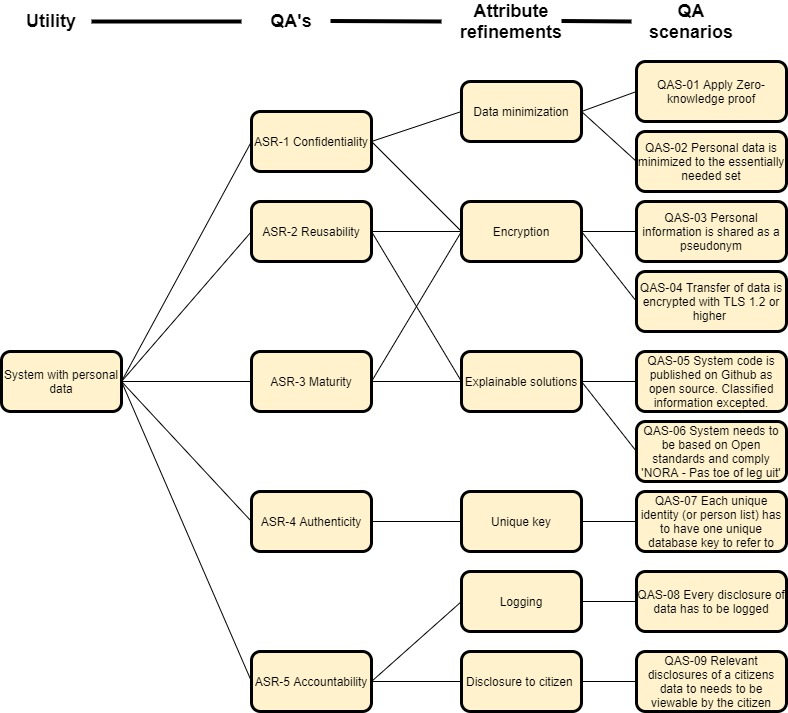
\includegraphics[width=14cm]{Decomposition of ASR and QAS-Utility Tree v2.jpg}\\
\caption{Decomposition of Architecturally significant requirements}
\label{fig:ASR1}
\end{figure}

\begin{table}[h!]
\centering
\begin{tabular}{||l l l||} 
 \hline
 Architectural Significant Requirement (ASR) & Business Goal(s) (BG) & Concern(s) (C)\\ [0.5ex] 
 \hline\hline
 \makecell{ASR-1 \\ Confidentiallity} & BG-03 & C-03 \\ 
 \hline
\makecell{ASR-2 \\ Reusability} & BG-01, BG-02 & C-01, C-02  \\
  \hline
\makecell{ASR-3 \\ Maturity} & BG-05 &  C-09  \\
  \hline
\makecell{ASR-4 \\ Authenticity} & BG-04 & C-04, C-05, C-06 \\
  \hline
\makecell{ASR-5 \\ Accountability} & BG-01 & C-10  \\ [1ex] 
 \hline
\end{tabular}
\caption{ASRs Plotted on business goals and concerns.}
\label{ASR_BG_C}
\end{table}

% \todo{
% This section provides a high-level outline of the proposed system or solution.
% It typically illustrates the system architecture or the interactions between the
% different solution components (via a “boxes-and-arrows” diagram) from a user’s
% perspective.
% }